\documentclass[notes=show,smaller,handout]{beamer}\usepackage[]{graphicx}\usepackage[]{color}
% maxwidth is the original width if it is less than linewidth
% otherwise use linewidth (to make sure the graphics do not exceed the margin)
\makeatletter
\def\maxwidth{ %
  \ifdim\Gin@nat@width>\linewidth
    \linewidth
  \else
    \Gin@nat@width
  \fi
}
\makeatother

\definecolor{fgcolor}{rgb}{0.345, 0.345, 0.345}
\newcommand{\hlnum}[1]{\textcolor[rgb]{0.686,0.059,0.569}{#1}}%
\newcommand{\hlstr}[1]{\textcolor[rgb]{0.192,0.494,0.8}{#1}}%
\newcommand{\hlcom}[1]{\textcolor[rgb]{0.678,0.584,0.686}{\textit{#1}}}%
\newcommand{\hlopt}[1]{\textcolor[rgb]{0,0,0}{#1}}%
\newcommand{\hlstd}[1]{\textcolor[rgb]{0.345,0.345,0.345}{#1}}%
\newcommand{\hlkwa}[1]{\textcolor[rgb]{0.161,0.373,0.58}{\textbf{#1}}}%
\newcommand{\hlkwb}[1]{\textcolor[rgb]{0.69,0.353,0.396}{#1}}%
\newcommand{\hlkwc}[1]{\textcolor[rgb]{0.333,0.667,0.333}{#1}}%
\newcommand{\hlkwd}[1]{\textcolor[rgb]{0.737,0.353,0.396}{\textbf{#1}}}%
\let\hlipl\hlkwb

\usepackage{framed}
\makeatletter
\newenvironment{kframe}{%
 \def\at@end@of@kframe{}%
 \ifinner\ifhmode%
  \def\at@end@of@kframe{\end{minipage}}%
  \begin{minipage}{\columnwidth}%
 \fi\fi%
 \def\FrameCommand##1{\hskip\@totalleftmargin \hskip-\fboxsep
 \colorbox{shadecolor}{##1}\hskip-\fboxsep
     % There is no \\@totalrightmargin, so:
     \hskip-\linewidth \hskip-\@totalleftmargin \hskip\columnwidth}%
 \MakeFramed {\advance\hsize-\width
   \@totalleftmargin\z@ \linewidth\hsize
   \@setminipage}}%
 {\par\unskip\endMakeFramed%
 \at@end@of@kframe}
\makeatother

\definecolor{shadecolor}{rgb}{.97, .97, .97}
\definecolor{messagecolor}{rgb}{0, 0, 0}
\definecolor{warningcolor}{rgb}{1, 0, 1}
\definecolor{errorcolor}{rgb}{1, 0, 0}
\newenvironment{knitrout}{}{} % an empty environment to be redefined in TeX

\usepackage{alltt}
%%%%%%%%%%%%%%%%%%%%%%%%%%%%%%%%%%%%%%%%%%%%%%%%%%%%%%%%%%%%%%%%%%%%%%%%%%%%%%%%%%%%%%%%%%%%%%%%%%%%%%%%%%%%%%%%%%%%%%%%%%%%%%%%%%%%%%%%%%%%%%%%%%%%%%%%%%%%%%%%%%%%%%%%%%%%%%%%%%%%%%%%%%%%%%%%%%%%%%%%%%%%%%%%%%%%%%%%%%%%%%%%%%%%%%%%%%%%%%%%%%%%%%%%%%%%
\usepackage{amssymb}
\usepackage{amsmath}
\usepackage{graphicx}
\usepackage{hyperref}
\usepackage{multimedia}
\usepackage{epstopdf}
\usepackage{color}

\setcounter{MaxMatrixCols}{10}
\newtheorem{remark}{Remark}[section]
\newtheorem{proposition}{Proposition}[section]
\newtheorem{interpretation}{Interpretation}[section]
\newtheorem{goal}{Goal}[section]
\newtheorem{statement}{Statement}[section]
\newtheorem{aes}{Aim \& Scope}[section]
\newtheorem{exercise}{Exercise}[section]
\renewcommand{\Pr}{P}

\newcommand{\mbf}[1]{\mathbf{#1}}
\newcommand{\beq}{\begin{equation}}
\newcommand{\eeq}{\end{equation}}
\newcommand{\bea}{\begin{eqnarray}}
\newcommand{\eea}{\end{eqnarray}}
\newcommand{\ba}{\begin{array}}
\newcommand{\ea}{\end{array}}
\newcommand{\bi}{\begin{itemize}}
\newcommand{\ei}{\end{itemize}}
\newcommand{\ben}{\begin{enumerate}}
\newcommand{\een}{\end{enumerate}}
\newcommand{\nn}{\nonumber}

\newenvironment{stepenumerate}{\begin{enumerate}[<+->]}{\end{enumerate}}
\newenvironment{stepitemize}{\begin{itemize}[<+->]}{\end{itemize} }
\newenvironment{stepenumeratewithalert}{\begin{enumerate}[<+-| alert@+>]}{\end{enumerate}}
\newenvironment{stepitemizewithalert}{\begin{itemize}[<+-| alert@+>]}{\end{itemize} }
\usetheme{Madrid}


%%%%%%%%%%%%%%%%%%%%%%%%%%%%%%%%%%%%%%%%%%%%%%%%%%%%%%%%%%%%%%%%%%%%%%%%%%%%%%%
% GSEM COLORS
%%%%%%%%%%%%%%%%%%%%%%%%%%%%%%%%%%%%%%%%%%%%%%%%%%%%%%%%%%%%%%%%%%%%%%%%%%%%%%%
\definecolor{darkGSEM}{RGB}{70,95,127}
\definecolor{darkGSEM2}{RGB}{40,80,150}
\definecolor{GSEM}{RGB}{96,121,153} % GSEM 10% lighter

%%% Global colors
\setbeamercolor*{palette primary}{use=structure,fg=white,bg=darkGSEM}
\setbeamercolor*{palette quaternary}{use=structure,fg=white,bg=darkGSEM!90}
\setbeamercolor{frametitle}{fg=white,bg=GSEM!80}

%%% TOC colors
\setbeamercolor{section in toc}{fg=darkGSEM}

%%% itemize colors
\setbeamertemplate{itemize items}[circle]
\setbeamercolor{itemize item}{fg=darkGSEM2}
\setbeamercolor{itemize subitem}{fg=darkGSEM2}
\setbeamercolor{itemize subsubitem}{fg=darkGSEM2}


%%% enumerate colors
\setbeamercolor{item projected}{fg=white,bg=GSEM}
\setbeamertemplate{enumerate item}{\insertenumlabel.}
\setbeamercolor{enumerate item}{fg=darkGSEM2}
\setbeamercolor{enumerate subitem}{fg=darkGSEM2}
\setbeamercolor{enumerate subsubitem}{fg=darkGSEM2}


\AtBeginSection[]
{
  \begin{frame}
    \frametitle{Outline}
    \tableofcontents[currentsection]
  \end{frame}
}

%%%%%%%%%%%%%%%%%%%%%%%%%%%%%%%%%%%%%%%%%%%%%%%%%%%%%%%%%%%%%%%%%%%%%%%%%%%%%%%%
\IfFileExists{upquote.sty}{\usepackage{upquote}}{}
\begin{document}


\title[S110015]{Probability 1}
\subtitle{Chapter 06 : Limit Theorems}
\author[Flores-Agreda, La Vecchia]{Dr. Daniel Flores-Agreda, \\[0.5em] \tiny{(based on the notes of Prof. Davide La Vecchia)}}
\date{Spring Semester 2021}

\begin{frame}
\titlepage
\end{frame}


\begin{frame}
\frametitle{Outline}
\tableofcontents
\end{frame}

\begin{frame}%
%EndExpansion

\frametitle{Sequences of Random Variables }

\begin{definition}
 A sequence of random variables is an ordered list of random variables
of the form%
\begin{equation*}
S_{1},S\,_{2},...,S_{n},...
\end{equation*}
where, in an abstract sense, the sequence is infinitely long.
\end{definition}

\vspace{0.4cm}

We would like to say something about how these random variables behave as $n$ gets larger and larger (i.e. as $n$
tends towards infinity, denoted by $n\rightarrow\infty$ )

\vspace{0.4cm}
The study of such limiting behaviour is commonly called a study of \color{blue}`asymptotics' \color{black} --- after the word asymptote used in standard calculus.

\end{frame}%
%EndExpansion

%TCIMACRO{\TeXButton{BeginFrame}{\begin{frame}}}%
%BeginExpansion
\begin{frame}%
%EndExpansion

\frametitle{Example: Bernoulli Trials and their sum}


Let $\tilde Z$ denote a dichotomous random variable with $\tilde Z\sim Bernoulli(p)$. A sequence of Bernoulli trials provides us with a sequence of values $\tilde Z_{1},\tilde Z_{2},...,\tilde Z_{n},...$ %where each $\tilde Z_{i}$ is such that
\begin{eqnarray*}
\Pr("Success")=\Pr \left( \tilde Z_{i}=1\right) = p & \text{and} & \Pr("Failure")=\Pr \left( \tilde Z_{i}=0\right)  = 1-p
\end{eqnarray*}
Now let
$$S_n=\sum_{s=1}^n \tilde Z_s,$$ the number of "Successes" in the first $n$ Bernoulli trials. This yields a new sequence of random variables
\begin{small}
\begin{eqnarray*}
S_{1} &=& \tilde Z_{1} \\
S_{2} &=&\left( \tilde Z_{1}+ \tilde Z_{2}\right)\\
&&\vdots  \\
S_{n} &=&\left( \tilde Z_{1}+ \tilde Z_{2}+\cdots + \tilde Z_{n}\right) = \sum_{i=1}^n \tilde Z_i
\end{eqnarray*}
\end{small}
This new sequence is such that $S_n\sim B(n,p)$ for each $n$.

\end{frame}%

\begin{frame}%
%EndExpansion

\frametitle{Example: Bernoulli Trials and their sum}


Now consider the sequence
$${P}_n=S_n/n,$$
for $n=1,2,\ldots$, corresponds to the proportion of `Successes'in the first $n$ Bernoulli trials.
\vspace{0.4cm}


It is natural to ask how the behaviour of  ${P}_n$ is related to the true probability of a `Success' ($p$).
\vspace{0.4cm}

%\item We can provide a reasonably complete description of the behaviour of $\bar{P}_n$:
%\begin{stepitemize}
%\item $\bar{P}_n\sim \frac{1}{n}Binomial(n,p)$,
%\item $E[\bar{P}_n]=p$ and $Var(\bar{P}_n)=p(1-p)/n$ for all $n$, and
%\item as $n\rightarrow\infty$ the probability distribution of
%$$
%\frac{\sqrt{n}(\bar{P}_n-p)}{\sqrt{p(1-p)}}
%$$
%is closely approximated by a standard normal.
%\end{stepitemize}

Specifically, the open question at this point is: \\
\vspace{0.3cm}
\begin{center}
\color{red} "Do these results imply that ${P}_n$ collapses onto the true $p$ as $n$ increases, and if
so, in what way?"  \color{black} \\ \vspace{0.3cm}
\end{center}
To gain a clue, let us consider the simulated values of ${P}_n$.

%\end{stepitemize}
\end{frame}%

\begin{frame}%
%EndExpansion

\frametitle{Example: Bernoulli Trials and limit behaviour}

\begin{figure}[ptb]\centering
\begin{tabular} {cc}
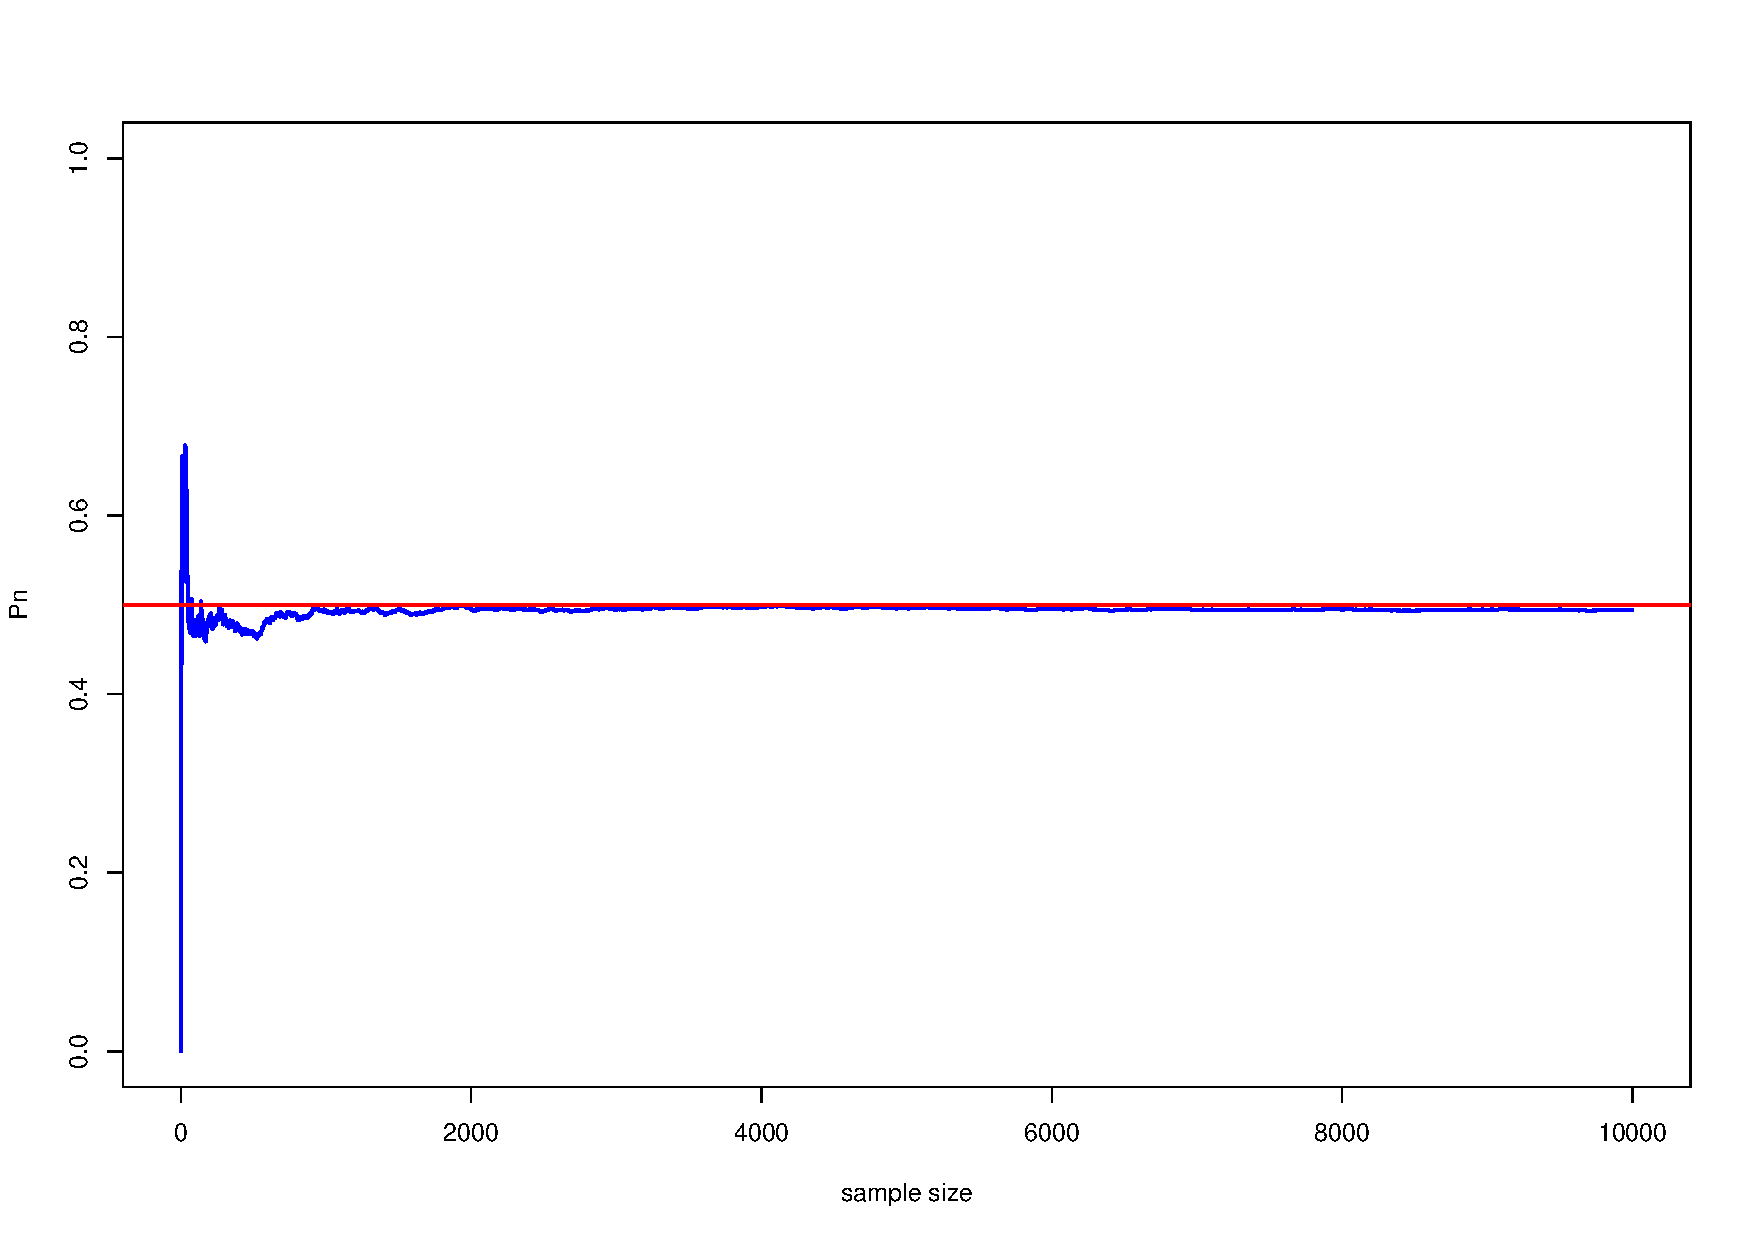
\includegraphics[height=1.56in, width=2.2in]{img/OneSample_Pn.pdf} &
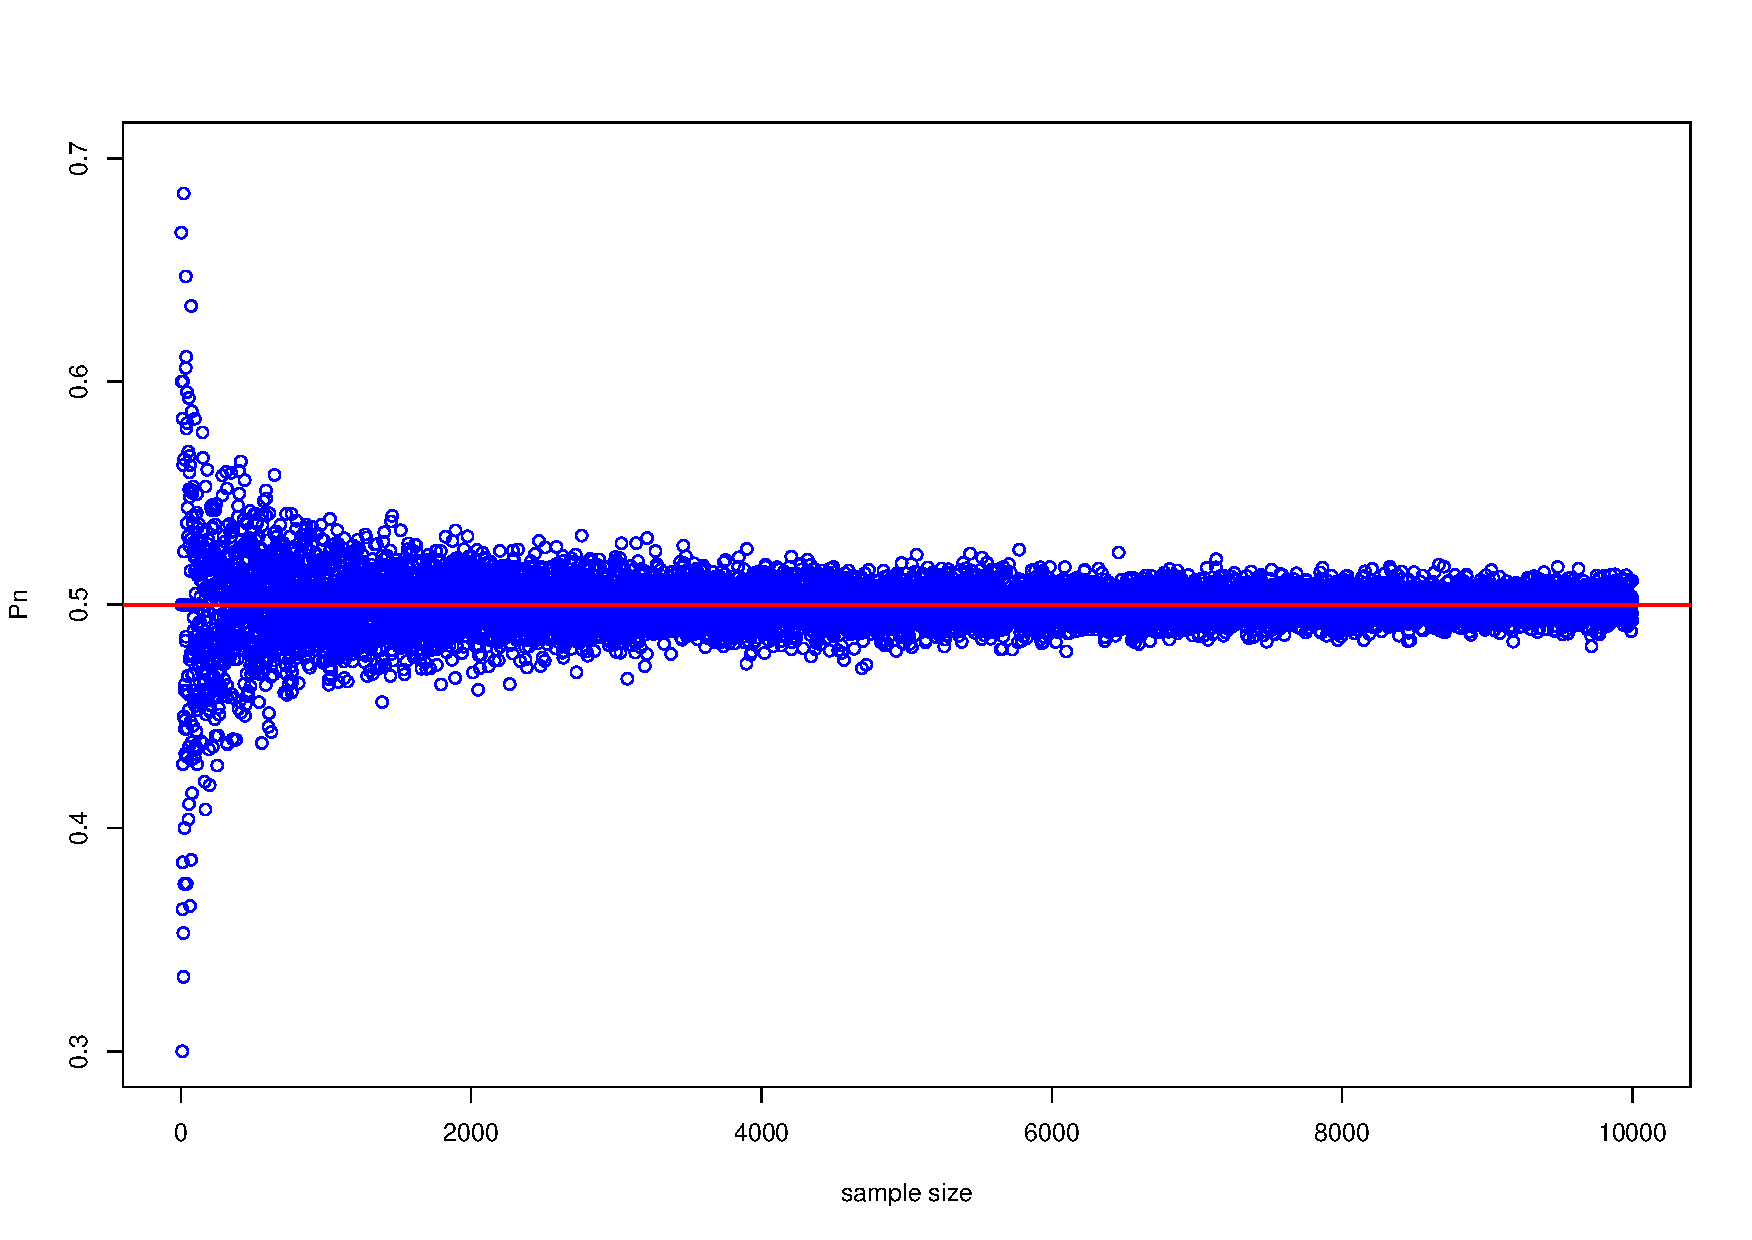
\includegraphics[height=1.56in, width=2.2in]{img/ManySamples_Pn.pdf} \\
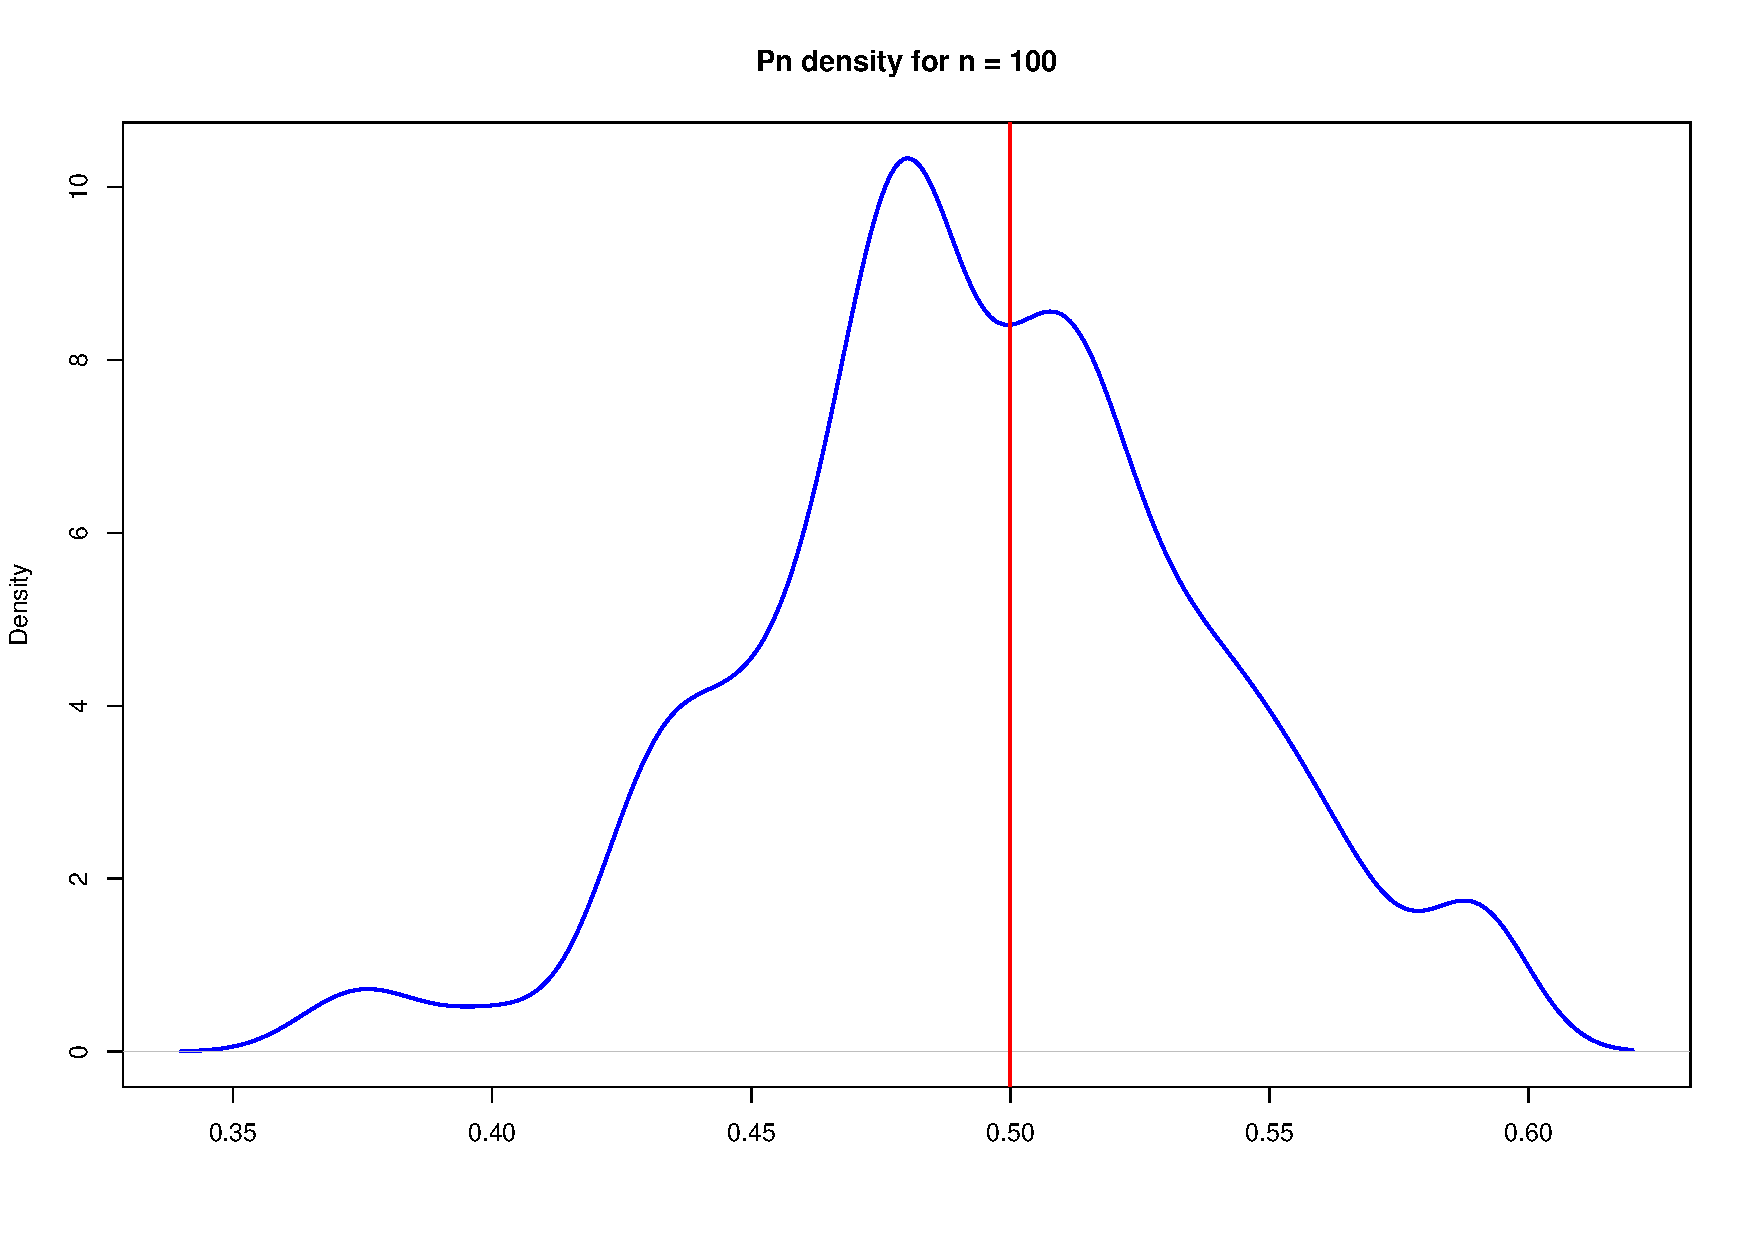
\includegraphics[height=1.56in, width=2.2in]{img/NonGauss_Pn.pdf} &
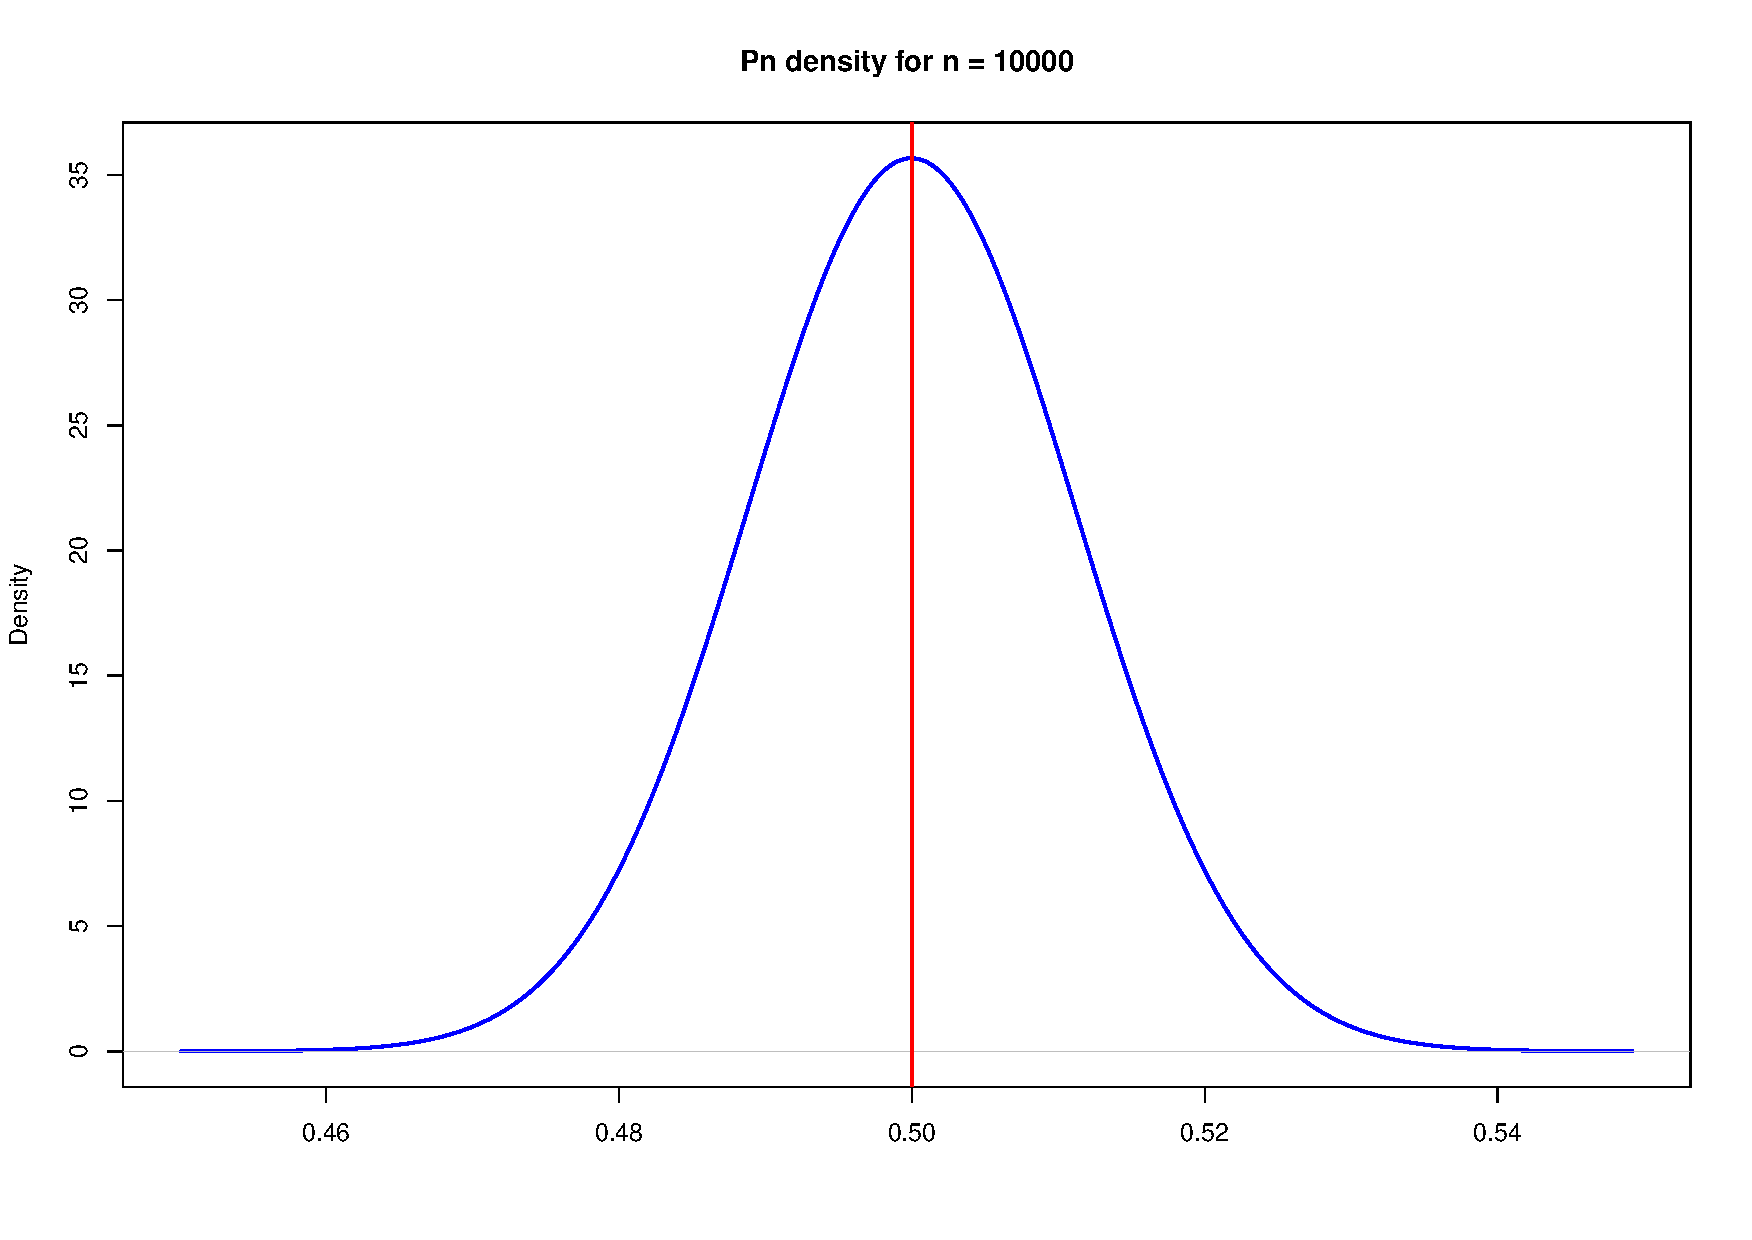
\includegraphics[height=1.56in, width=2.2in]{img/Gauss_Pn.pdf}
\end{tabular}
\end{figure}%


%TCIMACRO{\TeXButton{EndFrame}{\end{frame}}}%
%BeginExpansion
\end{frame}%
%EndExpansion


\begin{frame}%
%EndExpansion

\frametitle{Example: Bernoulli Trials and limit behaviour}

\begin{remark}
This numerical illustration leads us to suspect that there is a sense in which ${P}_n$ converges to $p$ --- notice that although the sequence is random, the `limiting' value here is a constant (i.e. is non-random).
\end{remark}

\vspace{1.5cm}

So, informally, we can claim that a sequence of random variables $X_{1},X_{2},...,X_{n},...$ is thought to
converge if the probability distribution of $X_{n}$ gets more and more concentrated around a single point as $n$ tends to infinity.
\end{frame}


%TCIMACRO{\TeXButton{BeginFrame}{\begin{frame}}}%
%BeginExpansion
\begin{frame}%
%EndExpansion

\frametitle{Convergence in Probability ($\overset{p}{\rightarrow }$)}

More formally,

\begin{definition}
A sequence of random variables $X_{1},X_{2},...,X_{n},...$ is said to \textbf{%
converge in probability} to a number $\alpha $ if for any arbitrary constant $\varepsilon >0$%
\begin{equation*}
\lim_{n\rightarrow \infty }\Pr \left( \left\vert X_{n}-\alpha \right\vert
>\varepsilon \right) =0
\end{equation*}
If this is the case, we write $X_{n}\overset{p}{\rightarrow }\alpha$ or $p\lim X_{n}=\alpha$. \\
\vspace{0.3cm}
A sequence of random variables $X_{1},X_{2},...,X_{n},...$ is said to \textbf{%
converge in probability} to a random variable $X$ if for any arbitrary constant $\varepsilon >0$%
\begin{equation*}
\lim_{n\rightarrow \infty }\Pr \left( \left\vert X_{n}-X \right\vert
>\varepsilon \right) =0\,,
\end{equation*}
written $X_{n}\overset{p}{\rightarrow }X$ or $p\lim(X_{n}-X)=0$.
\end{definition}
\end{frame}%
%EndExpansion

%TCIMACRO{\TeXButton{BeginFrame}{\begin{frame}}}%
%BeginExpansion
\begin{frame}%
%EndExpansion

\frametitle{Operational Rules for $\overset{p}{\rightarrow }$}
Let us itemize some rules. To this end, let $a$ be any (nonrandom) number so:

%\vspace{0.2cm}

\begin{stepitemize}
\item If $X_{n}\overset{p}{\rightarrow }%
\alpha $ then \vspace{0.3cm}
\begin{stepitemize}
\item $aX_{n}\overset{p}{\rightarrow }a\alpha $ and \vspace{0.3cm}
\item $a+X_{n}\overset{p}{\rightarrow }a+\alpha$,
\end{stepitemize}

\vspace{0.4cm}
\item If $X_{n}\overset{p}{\rightarrow }X $ then \vspace{0.3cm}
\begin{stepitemize}
\item $aX_{n}\overset{p}{\rightarrow }aX $ and \vspace{0.6cm}
\item $a+X_{n}\overset{p}{\rightarrow }a+X $
\end{stepitemize}

\vspace{0.4cm}
\item If $X_{n}\overset{p}{\rightarrow }\alpha $ and $Y_{n}\overset{p}{%
\rightarrow }\gamma $ then \vspace{0.3cm}
\begin{stepitemize}
\item $X_{n}Y_{n}\overset{p}{\rightarrow }\alpha \gamma$ and \vspace{0.3cm}
\item $X_{n}+Y_{n}\overset{p}{\rightarrow }\alpha +\gamma$.
\end{stepitemize}

\end{stepitemize}

\end{frame}%
%EndExpansion

%TCIMACRO{\TeXButton{BeginFrame}{\begin{frame}}}%
%BeginExpansion
\begin{frame}%
%EndExpansion

\frametitle{Operational Rules for $\overset{p}{\rightarrow }$}

\begin{stepitemize}
\item If $X_{n}\overset{p}{\rightarrow }X $ and $Y_{n}\overset{p}{%
\rightarrow }Y $ then  \vspace{0.3cm}

\begin{stepitemize}
\item $X_{n}Y_{n}\overset{p}{\rightarrow }X Y$ and  \vspace{0.3cm}

\item $X_{n}+Y_{n}\overset{p}{\rightarrow }X +Y$
\end{stepitemize}

 \vspace{0.6cm}

\item Let $g\left( x\right) $ be any (non-random) continuous function. If $%
X_{n}\overset{p}{\rightarrow }\alpha $ then
$$
g\left( X_{n}\right) \overset{p}{\rightarrow }g\left( \alpha \right),
$$
and if $X_{n}\overset{p}{\rightarrow }X $ then
$$g\left( X_{n}\right) \overset{p}{\rightarrow }g\left( X \right).
$$

\end{stepitemize}


%TCIMACRO{\TeXButton{EndFrame}{\end{frame}}}%
%BeginExpansion
\end{frame}%
%EndExpansion

%TCIMACRO{\TeXButton{BeginFrame}{\begin{frame}}}%
%BeginExpansion
\begin{frame}%
%EndExpansion

\frametitle{Convergence of Sample Moments as a motivation...}

Suppose $X_{1},X_{2},...,X_{n},...$ is a sequence of \textit{i.i.d.} random variables with common distribution $F_X(x)$ and moments $\mu_r=E
[X^r]$. At any given point along the sequence, $X_{1},X_{2},...,X_{n}$ constitutes a simple random sample of size $n$. \\

For each fixed sample size $n$, the $r$th sample moment is (using an obvious notation)
\begin{equation*}
M_{(r,n)}=\frac{1}{n}\left( X_{1}^r+X_{2}^r+\cdots +X_{n}^r\right)=\frac{1}{n}\sum_{s=1}^nX_s^r\,,
\end{equation*}
and we know that \vspace{0.25cm}
$$
E[M_{(r,n)}]=\mu_r\quad\text{and}\quad Var(M_{(r,n)})=\frac{1}{n}(\mu_{2}-\mu_1^2)\,.
$$
\vspace{0.25cm}

Now consider the sequence of sample moments $M_{(r,1)},M_{(r,2)},...,M_{(r,n)},...$ or, equivalently, $\{M_{(r,i)}\}_{i=1}^{n}$.


\end{frame}%

%%TCIMACRO{\TeXButton{BeginFrame}{\begin{frame}}}%
%%BeginExpansion
%\begin{frame}%
%%EndExpansion
%
%\frametitle{An informal example (continued)}
%
%\begin{stepitemize}
%\item The expected value of the sample mean is%
%\begin{eqnarray*}
%E\left[ \overline{X}_{n}\right]  &=&E\left[ \frac{1}{n}\left(
%X_{1}+X_{2}+\cdots +X_{n}\right) \right]  \\
%&=&\frac{1}{n}\left( E\left[ X_{1}\right] +E\left[ X_{2}\right] +\cdots +E%
%\left[ X_{n}\right] \right)  \\
%&=&\frac{1}{n}\left( \mu +\mu +\cdots +\mu \right) =\mu
%\end{eqnarray*}
%
%\item The variance of the sample mean is%
%\begin{eqnarray*}
%Var\left( \overline{X}_{n}\right)  &=&Var\left( \frac{1}{n}\left(
%X_{1}+X_{2}+\cdots +X_{n}\right) \right)  \\
%&=&\frac{1}{n^{2}}\left( Var\left( X_{1}\right) +Var\left( X_{2}\right)
%+\cdots +Var\left( X_{n}\right) \right)  \\
%&=&\frac{1}{n^{2}}\left( \sigma ^{2}+\sigma ^{2}+\cdots +\sigma ^{2}\right)
%\\
%&=&\frac{n\sigma ^{2}}{n^{2}}=\frac{\sigma ^{2}}{n}
%\end{eqnarray*}
%\end{stepitemize}
%
%%TCIMACRO{\TeXButton{EndFrame}{\end{frame}}}%
%%BeginExpansion
%\end{frame}%
%%EndExpansion

%TCIMACRO{\TeXButton{BeginFrame}{\begin{frame}}}%
%BeginExpansion
\begin{frame}%
%EndExpansion

\frametitle{Convergence of Sample Moments as a motivation...}

The distribution of $M_{(r,n)}$ (which is unknown because $F_X(x)$ has not been specified) is thus concentrated around $\mu_r $ for all $n$,
with a variance which tends to zero as $n$ increases. \\ \vspace{0.4cm}

So the distribution of $M_{(r,n)}$ becomes more and more concentrated around $\mu_r$ as $n
$ increases and therefore we might \color{blue}\emph{anticipate }\color{black} that
\begin{equation*}
M_{(r,n)}\overset{p}{\rightarrow }\mu_r.
\end{equation*}

\vspace{0.3cm}
In fact, this result follows from what is known as the \textbf{Weak Law of Large Numbers} (WLLN).
%\item N.B. If we define the sample MGF as
%$$
%\bar{M}_X(t)=\frac{1}{n}\sum_{s=1}^ne^{tX_s}=\sum_{r=0}^\infty M_{(r,n)}\frac{t^r}{r!}\,,
%$$
%then
%$$
%\bar{M}_X(t)-M_X(t)=\sum_{r=0}^\infty (M_{(r,n)}-\mu_r)\frac{t^r}{r!}\,.
%$$
%Using the operational rules for probability limits indicates that $p\lim\bar{M}_X(t)=M_X(t)$. This suggests \textit{estimating} $F_X(x)$ from "the data"!
%%\item But how can we formally prove this WLLN?
\end{frame}%

\begin{frame}%

\frametitle{The Weak Law of Large Numbers (WLLN)}

\begin{proposition}
 Let $X_{1},X_{2},...,X_{n},...$ be a sequence of \textit{i.i.d.} random variables with common probability distribution $F_X(x)$, and let $Y=h(X)$ be such that
\begin{eqnarray*}
E[Y]=E\left[ h(X)\right]  &=&\mu_Y  \\
Var(Y)=Var\left( h(X)\right)  &=&\sigma_Y ^{2}<\infty\,.
\end{eqnarray*}%
Set
$$
\overline{Y}_n=\frac{1}{n}\sum_{s=1}^nY_s\quad\text{where}\quad Y_s=h(X_s)\,,\quad s=1,\ldots,n\,.
$$
Then for any two numbers $\varepsilon$ and $\delta$ satisfying $\varepsilon>0$ and $0<\delta<1$
$$
\Pr \left( \left\vert \overline{Y}_{n}-\mu_Y \right\vert<\varepsilon \right)\geq 1-\delta
$$
for all $n>\sigma_Y^2/(\varepsilon^2\delta)$. Choosing both $\varepsilon$ and $\delta$ to be arbitrarily small implies that $p\lim_{n\rightarrow\infty}(\overline{Y}_{n}-\mu_Y)=0$, or equivalently
$\overline{Y}_{n}\overset{p}{\rightarrow }\mu_Y$.
\end{proposition}

%TCIMACRO{\TeXButton{EndFrame}{\end{frame}}}%
%BeginExpansion
\end{frame}%
%EndExpansion

%TCIMACRO{\TeXButton{BeginFrame}{\begin{frame}}}%
%BeginExpansion
\begin{frame}%
%EndExpansion

\frametitle{The WLLN and Chebyshev's Inequality}

\begin{stepitemize}
\item First note that $E[\overline{Y}_n]=\mu_Y$ and $Var(\overline{Y}_n)=\sigma_Y^2/n$.
\item Now, according to \textbf{Chebyshev's inequality}
\begin{eqnarray*}
\Pr \left( |\overline{Y}_{n}-\mu_Y| <\varepsilon\right)  &\geq &1-\frac{E\left[ \left(
\overline{Y}_{n}-\mu_Y \right) ^{2}\right] }{\varepsilon^{2}} \\
&=&1-\frac{\sigma_Y ^{2}/n}{\varepsilon^{2}} \\
&=&1-\frac{\sigma_Y ^{2}}{n\varepsilon^{2}}\geq 1-\delta
\end{eqnarray*}
for all $n>\sigma_Y^2/(\varepsilon^2\delta)$.
\item Thus the WLLN is proven, provided we can verify \textbf{Chebyshev's inequality}.
\item Note that by considering the limit as $n\rightarrow \infty $ we also have%
\begin{equation*}
\lim_{n\rightarrow \infty }\Pr \left( \left\vert \overline{Y}_{n}-\mu_Y\right\vert <\varepsilon\right) \geq \lim_{n\rightarrow \infty }\left( 1-\frac{\sigma^{2}}{n\varepsilon^{2}}\right) =1\,,
\end{equation*}
again implying that $\left( \overline{Y}_{n}-\mu_Y \right) \overset{p}{\rightarrow }0$.
\end{stepitemize}

%TCIMACRO{\TeXButton{EndFrame}{\end{frame}}}%
%BeginExpansion
\end{frame}%
%EndExpansion

%TCIMACRO{\TeXButton{BeginFrame}{\begin{frame}}}%
%BeginExpansion
\begin{frame}%
%EndExpansion

\frametitle{Chebyshev's (and Markov's) Inequality}

\begin{stepitemize}
\item \textbf{Chebychev's Inequality}: For any random variable $Z$ with mean $\mu_Z$ and variance $\sigma_Z^2<\infty$
\begin{equation*}
\Pr \left( \left\vert Z-\mu_Z\right\vert <r\sigma_Z\right) \geq 1-\frac{1 }{r^{2}}
\end{equation*}
for all $r>0$.
\begin{stepitemize}
\item Note that an equivalent expression is given by
\begin{equation}
\Pr \left( \left\vert Z-\mu_Z\right\vert \geq r\sigma_Z\right) \leq \frac{1 }{r^{2}} \label{Eq. C2}
\end{equation}
\item This inequality says that the probability that a random variable lies more than $r$ standard deviations away from its mean value is bounded above by $1/r^2$.
\end{stepitemize}
\item Chebychev's inequality is, in turn, a special case of Markov's inequality.
\item \textbf{Markov's inequality}: Let $Z$ be random variable and $h(z)$ a non-negative valued function for all $z\in \mathbb{R}$. Then
\begin{equation}
\Pr(h(Z)\geq \zeta)\leq \frac{E[h(Z)]}{\zeta}\quad\text{for all}\,\zeta>0. \label{Eq. M1}
\end{equation}
\end{stepitemize}

%TCIMACRO{\TeXButton{EndFrame}{\end{frame}}}%
%BeginExpansion
\end{frame}%
%EndExpansion

%TCIMACRO{\TeXButton{BeginFrame}{\begin{frame}}}%
%BeginExpansion
\begin{frame}%
%EndExpansion

\frametitle{Chebyshev's (and Markov's) Inequality}

\begin{stepitemize}
\item To verify Markov's inequality, observe that
\begin{eqnarray*}
E[h( Z)]&=&\int_{-\infty }^{\infty }h(z) f_{Z}\left(z\right)dz\\
&=&\int_{\{z:h(z)\geq\zeta\}}h(z) f_{Z}\left(z\right) dz+
\int_{\{z:h(z)<\zeta\}}h(z) f_{Z}\left(z\right) dz \\
&\geq&\int_{\{z:h(z)\geq\zeta\}}h(z) f_{Z}\left(z\right) dz\\
&\geq&\int_{\{z:h(z)\geq\zeta\}}\zeta f_{Z}\left(z\right)dz=\zeta\Pr(h(Z)\geq\zeta)\,,
\end{eqnarray*}
giving the desired result on division by $\zeta$.
\item Chebyshev's inequality now follows as a direct corollary of Markov's inequality on taking $h(z)=(z-\mu_Z)^2$ and $\zeta=r^2\sigma_Z^2$.
%\item Chebychev's inequality
It can be used to construct crude bounds on the probabilities associated with deviations of a random variable from its mean.
%But we are more often interested in more precise evaluations.

\end{stepitemize}

%TCIMACRO{\TeXButton{EndFrame}{\end{frame}}}%
%BeginExpansion
\end{frame}%
%EndExpansion

\begin{frame}%
%EndExpansion

\frametitle{Example: Markov's Inequality}

\begin{example}

\textbf{Q.} On the A2 highway (in the Luzern Canton), the speed limit is $80$ Km/h. Most drivers are not driving so fast and the average speed on the high way is $70$ Km/h.
If $Z$ denotes a randomly chosen driver's speed, what is the probability that such a person is driving faster than the speed limit? \\
\vspace{1cm}
\textbf{A.} Since we do not have the whole distribution of $Z$, but we have only limited info (i.e. we know $E[Z]=70$ Km/h), we have to resort on Markov's inequality. So using (\ref{Eq. M1}) we obtain an upper bound to the probability:
$$
P(Z \geq 80) \leq \frac{70}{80} = 0.875.
$$


\end{example}
\end{frame}%
%EndExpansion

\begin{frame}%
%EndExpansion



\frametitle{Example: Chebyshev's Inequality}

\begin{example}

\textbf{Q.} On the A2 highway (in the Luzern Canton), the speed limit is $80$ Km/h. Most drivers are not driving so fast and the average speed on the high way is $70$ Km/h, \textbf{with variance $9$ $(Km/h)^2$}.
If $Z$ denotes a randomly chosen driver's speed, what is the probability that such a person is driving faster than the speed limit? \\
\vspace{0.25cm}
\textbf{A.} Since we do not have the whole distribution of $Z$, but we have only limited info (i.e. we know $E[Z]=70$ Km/h \textbf{AND} $V(Z)=9$ $(Km/h)^2$), we have to resort on Chebyshev's inequality and give an upper bound to the probability. Thus,
\begin{small}
\begin{eqnarray*}
P( Z \geq 80) &=& P( Z - E[Z]\geq 80 - 70) \\ &\leq& P(\vert Z-E[Z] \vert \geq 10) \leq  P\left( \frac{\vert Z-E[Z] \vert }{\sqrt{V(Z)}}\geq \frac{10}{\sqrt{9}}\right)
\end{eqnarray*}
\end{small}

Using (\ref{Eq. C2}), with $r=\frac{10}{3}$ and $\sigma_Z= 3$, we finally get
\begin{small}
\begin{eqnarray*}
P( Z \geq 80) \leq P\left(\Big\vert Z-E[Z] \Big\vert \geq \left(\frac{10}{3}\right) {3}\right) \leq \frac{1}{\frac{10^2}{3^2}} \leq \frac{9}{100} \leq 0.09
\end{eqnarray*}
\end{small}

\end{example}

\end{frame}%


\begin{frame}%

\frametitle{A remark about Chebyshev's Inequality}

\begin{remark}
Chebichev's inequality can be rewirtten in a different way. \\

Indeed, for any random variable $Z$ with mean $\mu_Z$ and variance $\sigma_Z^2<\infty$
\begin{equation}
\Pr \left( \left\vert Z-\mu_Z\right\vert \geq \varepsilon \right) \leq \frac{E[Z-\mu_Z]^2}{\varepsilon^{2}} = \frac{\sigma_Z^2}{\varepsilon^{2}}. \label{Eq. C3}
\end{equation}

 It's easy to check  that Eq. (\ref{Eq. C3}) coincides with Eq. (\ref{Eq. C2}), setting in Eq. (\ref{Eq. C3})

 $$
 \varepsilon = r \sigma_Z.
 $$

 Do the check as an exercise!!
\end{remark}

\end{frame}%


%%TCIMACRO{\TeXButton{BeginFrame}{\begin{frame}}}%
%%BeginExpansion
%\begin{frame}%
%%EndExpansion
%
%\frametitle{Proof of Chebyshev's inequality (continuous case)}
%
%\begin{stepitemize}
%\item We can rewrite the RHS of Chebyshev's inequality as
%\begin{eqnarray*}
%1-\frac{E\left( Z^{2}\right) }{t^{2}} &=&E\left[ 1-\frac{Z^{2}}{t^{2}}\right]
%\\
%&=&\int_{-\infty }^{\infty }\left( 1-\frac{z^{2}}{t^{2}}\right) f_{Z}\left(
%z\right) dz \\
%&=&\int_{-\infty }^{-t}\left( 1-\frac{z^{2}}{t^{2}}\right) f_{Z}\left(
%z\right) dz \\
%&&+\int_{-t}^{t}\left( 1-\frac{z^{2}}{t^{2}}\right) f_{Z}\left( z\right) dz
%\\
%&&+\int_{t}^{\infty }\left( 1-\frac{z^{2}}{t^{2}}\right) f_{Z}\left(
%z\right) dz
%\end{eqnarray*}
%
%\begin{stepitemize}
%\item i.e. just break up the integral into three parts
%\end{stepitemize}
%\end{stepitemize}
%
%%TCIMACRO{\TeXButton{EndFrame}{\end{frame}}}%
%%BeginExpansion
%\end{frame}%
%%EndExpansion

%%TCIMACRO{\TeXButton{BeginFrame}{\begin{frame}}}%
%%BeginExpansion
%\begin{frame}%
%%EndExpansion
%
%\frametitle{Proof of Chebyshev's inequality (continued)}
%
%\begin{stepitemize}
%\item Notice that both of the outer integrals are non-positive,
%
%\begin{stepitemize}
%\item i.e.%
%\begin{equation*}
%\int_{-\infty }^{-t}\left( 1-\frac{z^{2}}{t^{2}}\right) f_{Z}\left( z\right)
%dz\leq 0
%\end{equation*}
%
%\item and%
%\begin{equation*}
%\int_{t}^{\infty }\left( 1-\frac{z^{2}}{t^{2}}\right) f_{Z}\left( z\right)
%dz\leq 0
%\end{equation*}
%
%\item since in both cases $\left( 1-\frac{z^{2}}{t^{2}}\right) \leq 0$
%\end{stepitemize}
%
%\item And so
%\begin{eqnarray*}
%E\left[ 1-\frac{Z^{2}}{t^{2}}\right]  &=&\int_{-t}^{t}\left( 1-\frac{z^{2}}{%
%t^{2}}\right) f_{Z}\left( z\right) dz+\text{something negative} \\
%&\leq &\int_{-t}^{t}\left( 1-\frac{z^{2}}{t^{2}}\right) f_{Z}\left( z\right)
%dz
%\end{eqnarray*}
%\end{stepitemize}
%
%%TCIMACRO{\TeXButton{EndFrame}{\end{frame}}}%
%%BeginExpansion
%\end{frame}%
%%EndExpansion

%%TCIMACRO{\TeXButton{BeginFrame}{\begin{frame}}}%
%%BeginExpansion
%\begin{frame}%
%%EndExpansion
%
%\frametitle{Proof of Chebyshev's inequality (continued)}
%
%\begin{stepitemize}
%\item So therefore we have that%
%\begin{eqnarray*}
%E\left[ 1-\frac{Z^{2}}{t^{2}}\right]  &\leq &\int_{-t}^{t}\left( 1-\frac{%
%z^{2}}{t^{2}}\right) f_{Z}\left( z\right) dz \\
%&=&\int_{-t}^{t}f_{Z}\left( z\right) dz-\int_{-t}^{t}\frac{z^{2}}{t^{2}}%
%f_{Z}\left( z\right) dz \\
%&=&\Pr \left( -t<Z<t\right) -\text{something positive} \\
%&\leq &\Pr \left( -t<Z<t\right)
%\end{eqnarray*}
%
%\item and hence Chebyshev's inequality holds
%\end{stepitemize}
%
%%TCIMACRO{\TeXButton{EndFrame}{\end{frame}}}%
%%BeginExpansion
%\end{frame}%
%%EndExpansion
%

%TCIMACRO{\TeXButton{BeginFrame}{\begin{frame}}}%
%BeginExpansion
\begin{frame}%
%EndExpansion

\frametitle{Convergence in Distribution}

\begin{definition}
Consider, therefore, a sequence of random variables $X_{1},X_{2},...,X_{n},...$ with corresponding CDFs $F_{X_{1}}\left( x\right) ,F_{X_{2}}\left( x\right),...,F_{X_{n}}\left(x\right) ,...$. We say that the sequence $X_{1},X_{2},...,X_{n},...$ \textbf{converges in distribution} to the random variable $X$, having probability distribution $F_X(x)$, if and only if
\begin{equation*}
\lim_{n\rightarrow \infty }F_{X_n}\left( x\right) =F_{X}\left( x\right)
\end{equation*}
at all points $x$ where $F_{X}\left( x\right) $ is continuous. In this case we write $X_{n}\overset{D}{\rightarrow }X$
\end{definition}
\end{frame}%



\begin{frame}%

\frametitle{Some Operational Rules for $\overset{D}{\rightarrow }$}

\begin{stepitemize}

\item If $p\lim_{n\rightarrow\infty}(X_n-X)=0$ then $X_{n}\overset{D}{\rightarrow }X$. \vspace{0.3cm}
\item Let $a$ be any real number. If $X_{n}\overset{D}{\rightarrow }X$, then
$aX_{n}\overset{D}{\rightarrow }aX$ \vspace{0.6cm}

\item If $Y_{n}\overset{p}{\rightarrow }\phi $ and $X_{n}\overset{D}{%
\rightarrow }X$, then \vspace{0.3cm}

\begin{stepitemize}
\item $Y_{n}X_{n}\overset{D}{\rightarrow }\phi X,$ and \vspace{0.3cm}

\item $Y_{n}+X_{n}\overset{D}{\rightarrow }\phi +X$
\end{stepitemize} \vspace{0.6cm}

\item If $X_{n}\overset{D}{\rightarrow }X$ and $g\left( x\right) $ is any
continuous function, then $g\left( X_{n}\right) \overset{D}{\rightarrow }%
g\left( X\right) $ \vspace{0.6cm}

%\item If $Y_{n}\overset{D}{\rightarrow }Y$ and $X_{n}\overset{D}{\rightarrow
%}X$, then

%\begin{stepitemize}
%\item $Y_{n}X_{n}\overset{D}{\rightarrow }YX,$ and
%
%\item $Y_{n}+X_{n}\overset{D}{\rightarrow }Y +X$
%\end{stepitemize}
\end{stepitemize}

%TCIMACRO{\TeXButton{EndFrame}{\end{frame}}}%
%BeginExpansion
\end{frame}


\begin{frame}%
%EndExpansion

\frametitle{Examples: Poisson and Normal Approximations to the Binomial Distribution}

\begin{example}
Suppose $X_{1},X_{2},...,X_{n},...$ is a sequence of independent
random variables where $X_n\sim B(n,p)$ with probability of "Success" $p$.\bigskip

\begin{stepitemize}

\item We already know that, if $p=\lambda/n$, where $\lambda>0$ is fixed, then as $n$ goes to infinity, $F_{X_{n}}\left( x\right) $ converges to
the probability distribution of a \color{blue}$Poisson\left( \lambda \right) $ \color{black} random variable. So, $X_{n}\overset{D}{\rightarrow }X$, where $X\sim Poisson\left(\lambda \right) $\bigskip

\item Now consider another case. If $p$ is fixed, the probability distribution of
\begin{equation*}
Y_{n}=\frac{X_{n}-np}{\sqrt{np\left( 1-p\right) }}
\end{equation*}
converges, as $n$ goes to infinity, to that of a \color{blue}standard Normal \color{black} random variable [Theorem of De Moivre-Laplace]. So, $Y_
{n}\overset{D}{\rightarrow }Y$, where $Y\sim \mathcal{N}\left(0,1\right) $.

\end{stepitemize}
\end{example}
\end{frame}%

\begin{frame}%

\frametitle{Example cont'd (visualize $Y_{n}$)}

\begin{example}


\begin{figure}[ptb]\centering
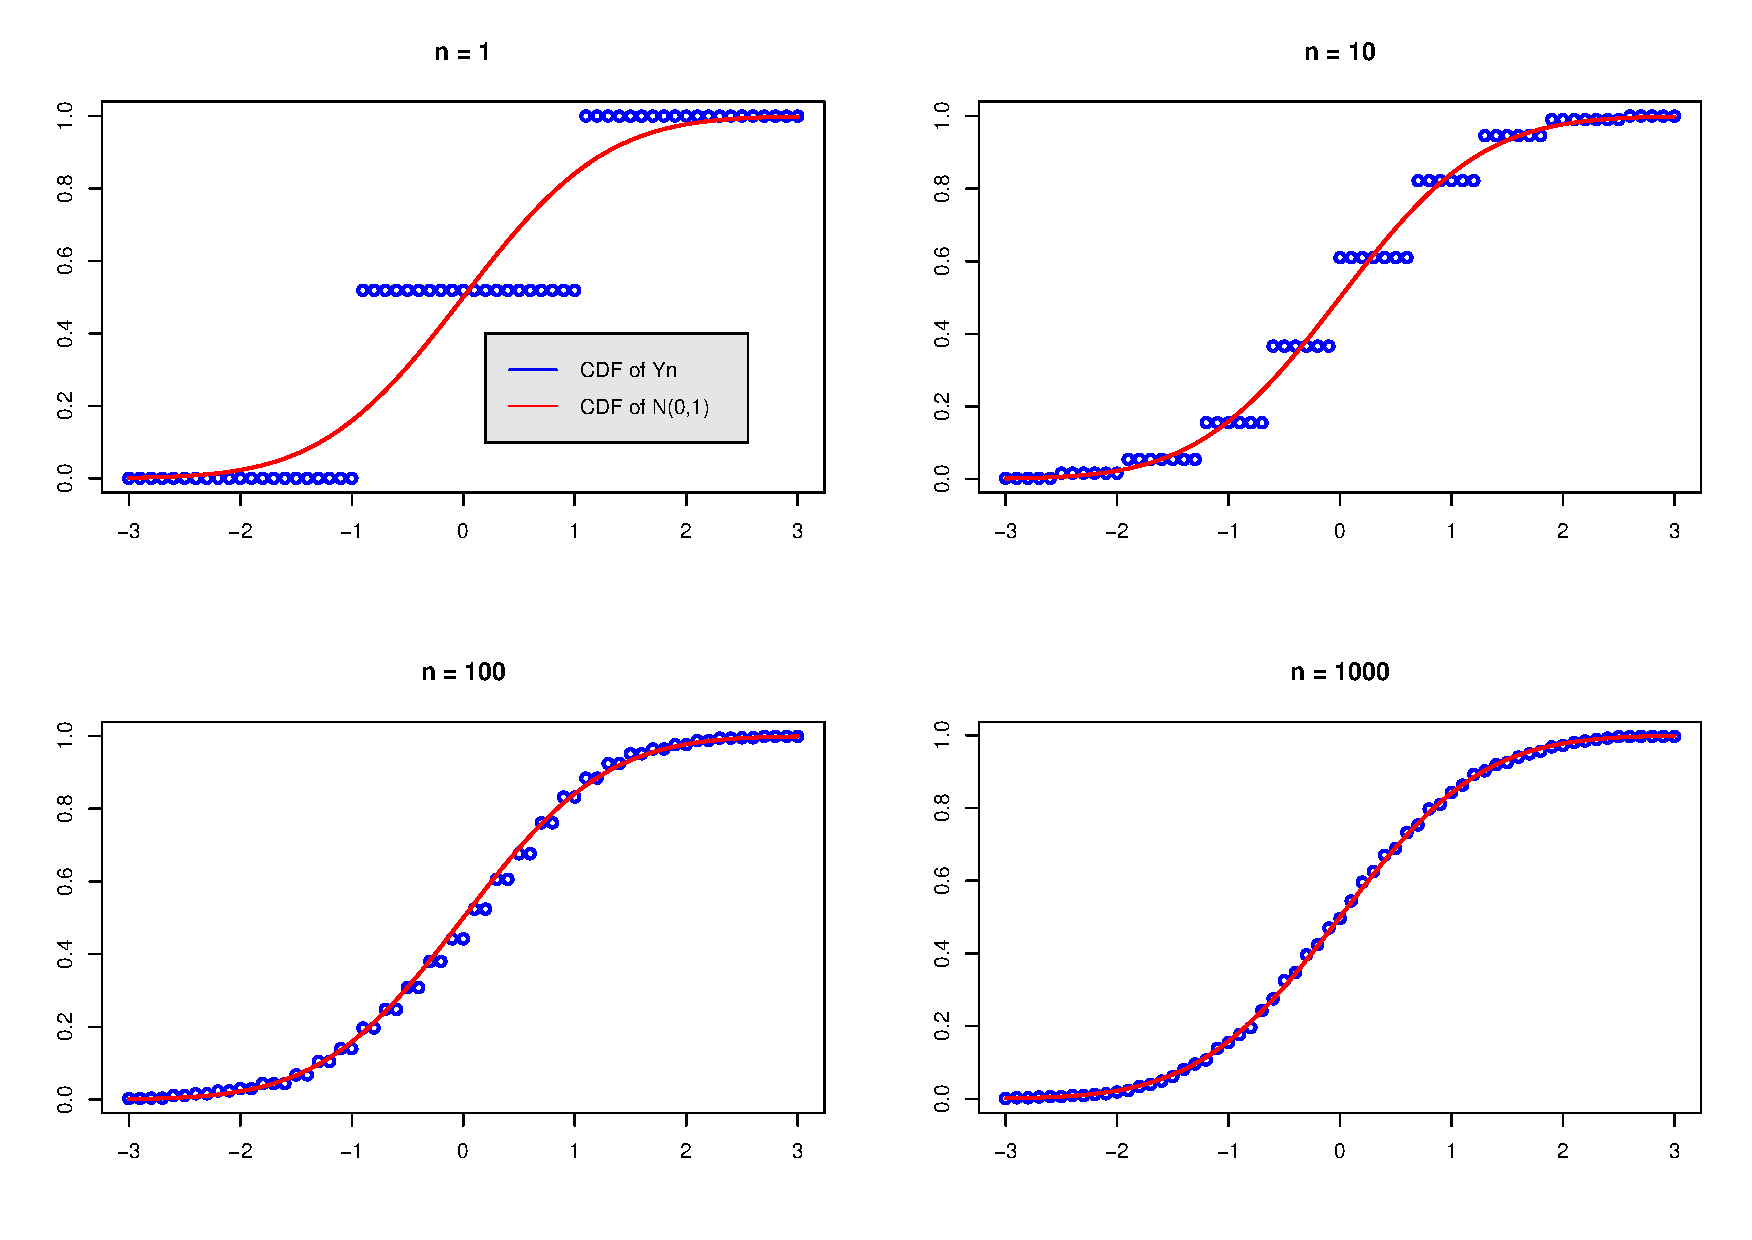
\includegraphics[height=2.9in, width=4in]{img/CDF_Rplot.pdf}%
\end{figure}%



\end{example}
\end{frame}%



\begin{frame}%
\frametitle{Example [convergence to an exp r.v.]}

\begin{example}
Let us consider a sequence of continuous r.v.'s $X_1, X_2, ..., X_n,...$, where $X_n$ has range $(0, n]$, for $n > 0$ and CDF
$$
F_{X_n} (x) = 1- \left( 1- \frac{x}{n} \right)^n,  \ \ 0<x\leq n.
$$
Then, as $n \to \infty$, the limiting support is $(0,\infty)$, and $\forall x >0$, we have
$$
F_{X_n} (x)  \to F_X(x) = 1 - e^{-x}
$$
which is the CDF of an exponential r.v. (at all continuity points). \vspace{0.5cm}

So, we conclude that $X_n$ convergences in distribution to an exponential r.v., that is
$$
X_n \overset{D}{\rightarrow } X, \quad X \sim \exp(1).
$$

\end{example}


\end{frame}%


\begin{frame}%
%EndExpansion

\frametitle{The Central Limit Theorem (CLT)}
The following theorem is often said to be one of the most important results. Its significance lies in the fact that it allows accurate probability calculations to be made without knowledge of the underlying distributions!

\begin{theorem} Let $X_{1},X_{2},...,X_{n},...$ be a sequence of \textit{i.i.d.} random variables and let $Y=h(X)$ be such that
\begin{eqnarray*}
E[Y]=E\left[ h(X)\right]  &=&\mu_Y  \\
Var(Y)=Var\left( h(X)\right)  &=&\sigma_Y ^{2}<\infty\,.
\end{eqnarray*}%
Set
$$
\overline{Y}_n=\frac{1}{n}\sum_{s=1}^nY_s\quad\text{where}\quad Y_s=h(X_s)\,,\quad s=1,\ldots,n\,.
$$
Then (under quite general regularity conditions)%
\begin{equation*}
\frac{\sqrt{n}\left( \overline{Y}_{n}-\mu_Y \right) }{\sigma_Y }\overset{D}{%
\rightarrow }N\left( 0,1\right).
\end{equation*}
\end{theorem}
\end{frame}%


\begin{frame}%
\frametitle{CLT: sum of Bernoulli rvs (from Kuonen)}
\begin{figure}[ptb]\centering
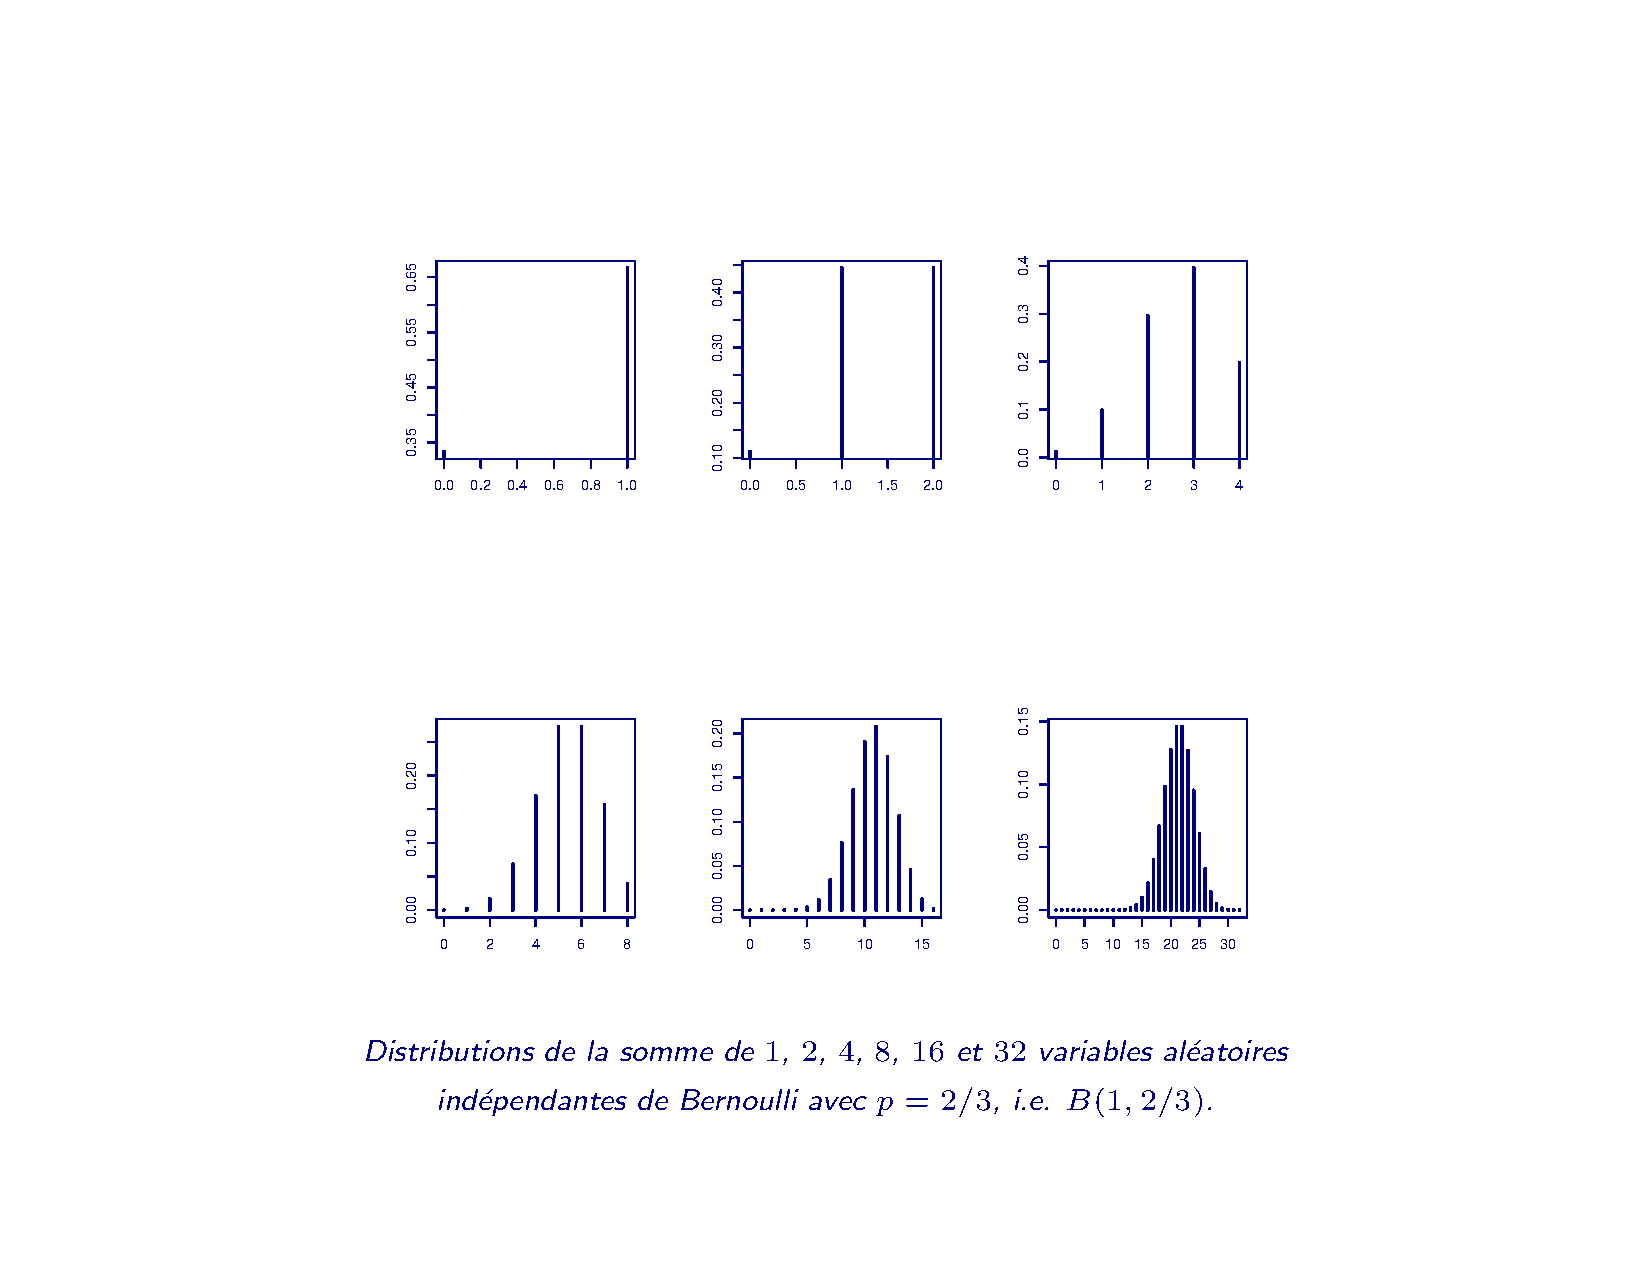
\includegraphics[height=3in, width=3.8in]{img/Bernoulli.pdf}%
\end{figure}%
\end{frame}%

%\begin{frame}%
%\begin{figure}[ptb]\centering
%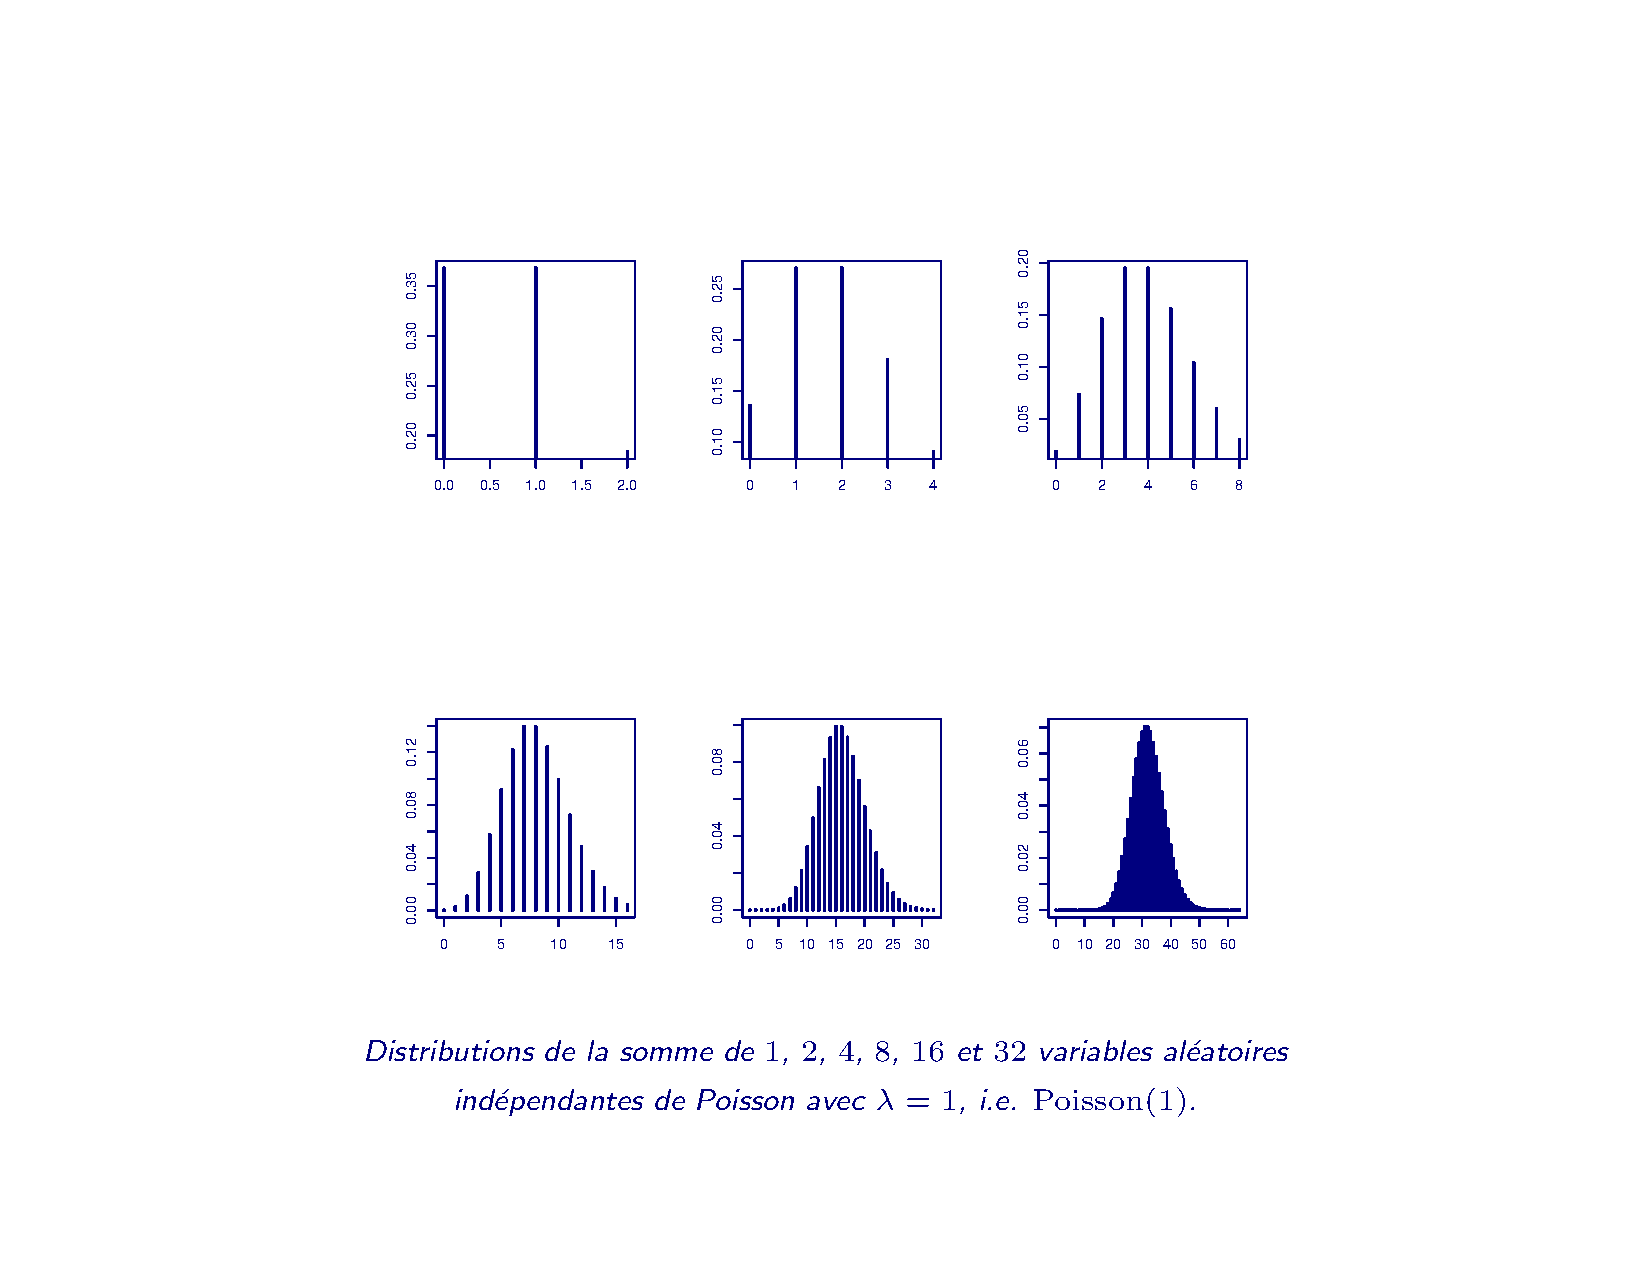
\includegraphics[height=3in, width=3.6in]{img/Poisson.pdf}%
%\end{figure}%
%\end{frame}%

\begin{frame}%
\frametitle{CLT: sum of Exp rvs (from Kuonen)}

\begin{figure}[ptb]\centering
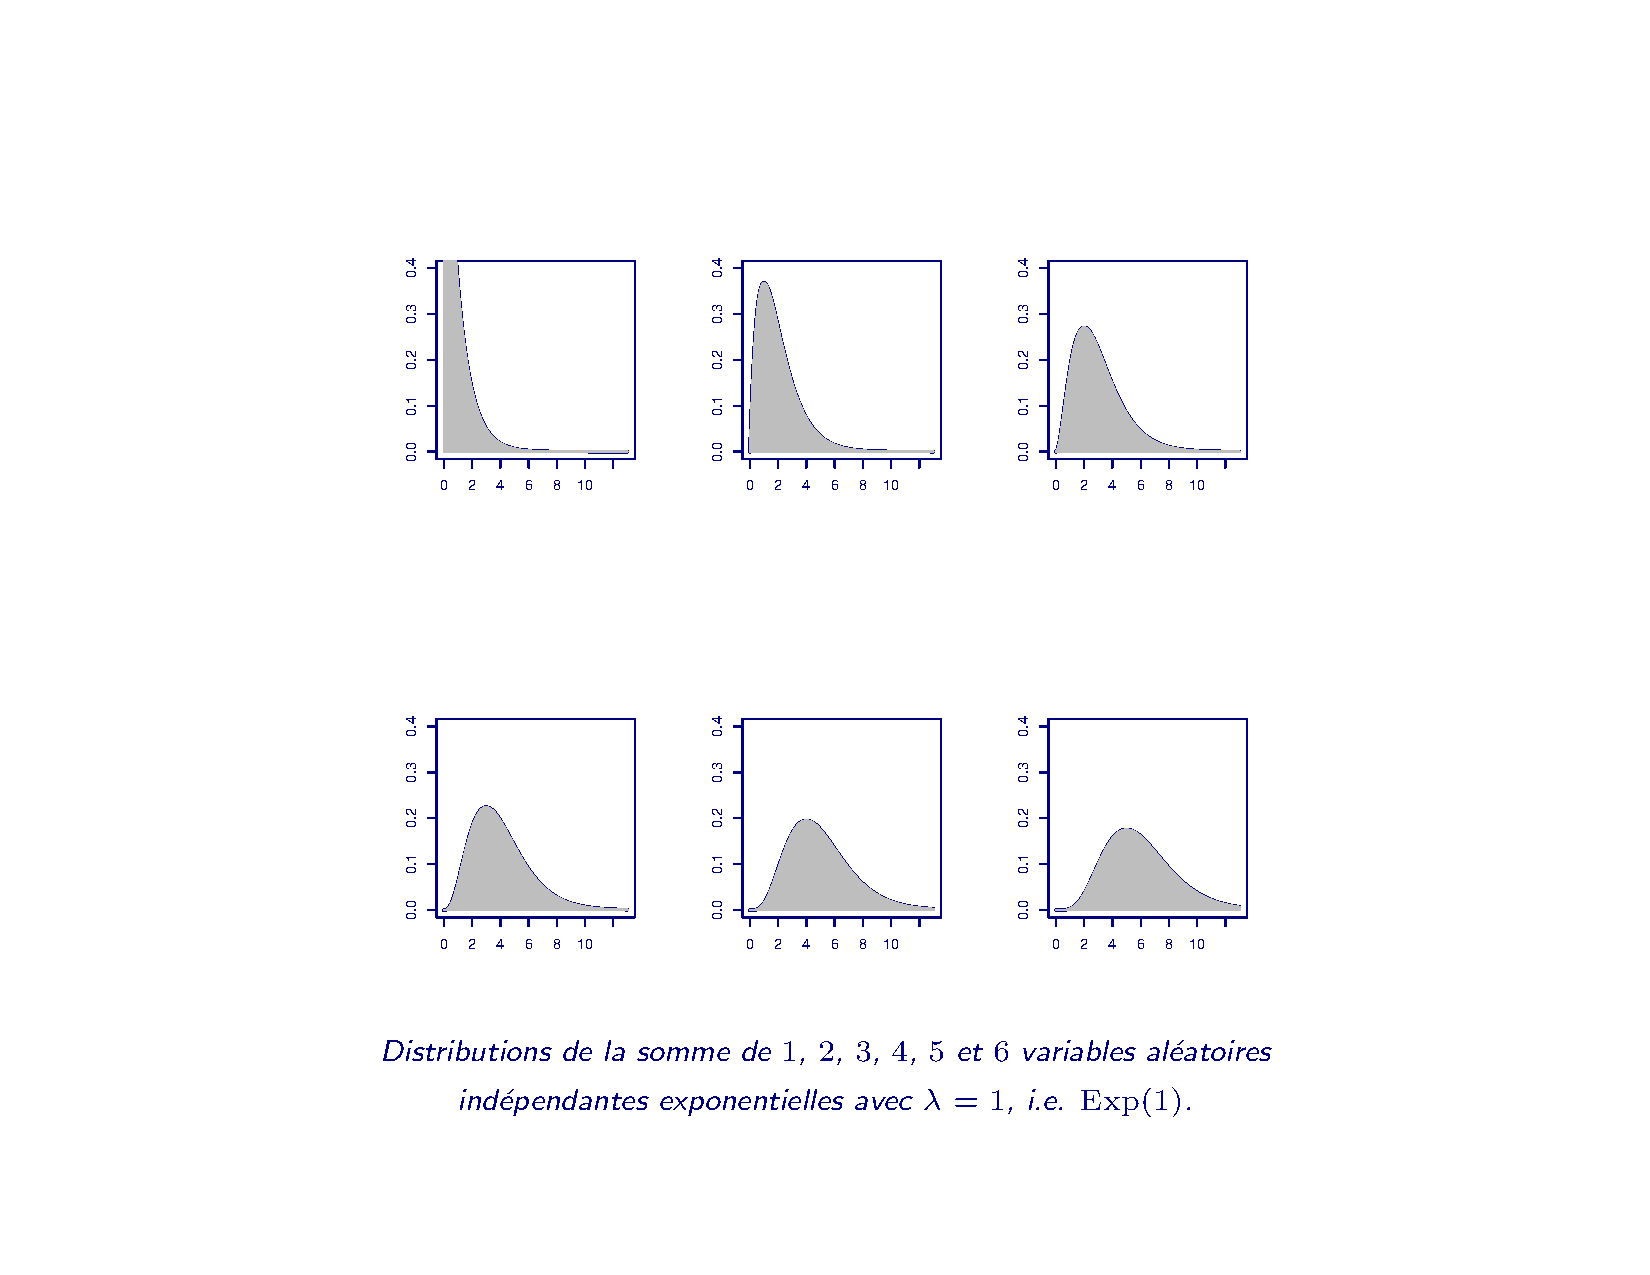
\includegraphics[height=3.2in, width=3.8in]{img/Exp.pdf}%
\end{figure}%
\end{frame}%


\begin{frame}%

\frametitle{The Central Limit Theorem (CLT)}

\begin{remark}
Several generalizations of this statement are available. For instance, one can state a CLT for data which are independent but NOT identically distributed. Another possibility is to define a CLT for data which are NOT independent, namely for dependent data --- for this you need to attend my course about Time Series, in the Fall semester at the Master in Statistics at University of Geneva !!!!
\end{remark}

\end{frame}%



\end{document}
